\documentclass[border=4pt]{standalone}
\usepackage{fontspec}
\setmainfont{DMSans9pt}[Path=../../fonts/, Extension=.ttf, UprightFont=*-Regular, BoldFont=*-Bold, ItalicFont=*-Italic, BoldItalicFont=*-BoldItalic]
\setsansfont{DMSans9pt}[Path=../../fonts/, Extension=.ttf, UprightFont=*-Regular, BoldFont=*-Bold, ItalicFont=*-Italic, BoldItalicFont=*-BoldItalic]
\usepackage{amsmath,amssymb,xcolor}
\usepackage{tikz}
\usetikzlibrary{arrows.meta,positioning,shapes.geometric,shapes.misc,fit,backgrounds,calc,decorations.pathreplacing,shadows}
\definecolor{cTwo}{HTML}{4C72B0}
\definecolor{cOne}{HTML}{DD8452}
\definecolor{cDetr}{HTML}{55A868}
\definecolor{cOvd}{HTML}{8172B3}
\definecolor{cAgent}{HTML}{C44E52}
\definecolor{cEdge}{HTML}{937860}
\definecolor{cApp}{HTML}{DA8BC3}
\definecolor{cData}{HTML}{4C9BB0}

\makeatletter
\def\refmap#1#2{\expandafter\def\csname rm@#1\endcsname{#2}}
\def\rm@ref#1{\csname rm@#1\endcsname}
\renewcommand{\ref}{\@ifstar\rm@ref\rm@ref}
\renewcommand{\eqref}[1]{(\csname rm@#1\endcsname)}
\makeatother

\refmap{eq:ciou}{10}\refmap{eq:detector}{1}\refmap{eq:dfl}{11}\refmap{eq:giou}{9}\refmap{eq:glip}{17}\refmap{eq:grpo}{20}\refmap{eq:infonce}{15}\refmap{eq:mllm-box}{19}\refmap{eq:ovd}{2}\refmap{eq:reparam}{18}\refmap{eq:roialign}{6}\refmap{eq:rpn}{5}\refmap{eq:siglip}{16}\refmap{eq:tal}{8}\refmap{sec:agentic}{5}\refmap{sec:closed}{3}\refmap{sec:manufacturing}{7.1}\refmap{sec:mllm-direct}{5.1}\refmap{sec:mllm-rl}{5.2}\refmap{sec:mllm-tools}{5.3}\refmap{sec:ovd}{4}\refmap{sec:ovd-distill}{4.2}\refmap{sec:ovd-grounding}{4.3}\refmap{sec:ovd-owl}{4.4}\refmap{sec:ovd-rt}{4.5}\refmap{sec:ovd-unified}{4.6}\refmap{sec:twostage}{3.1}\refmap{sec:vlfound}{4.1}\refmap{sec:yolo}{3.3}\refmap{tab:yolo}{4}
%% ---------- illustrative scene thumbnails (drawn, not photographs); origin = lower-left, size 2.4 x 1.7
\definecolor{pcbG}{HTML}{2E7D4F}\definecolor{pcbD}{HTML}{1F5A39}\definecolor{chipK}{HTML}{2B2B2B}
\definecolor{soil}{HTML}{8B6B4A}\definecolor{soilD}{HTML}{6E5238}\definecolor{crop}{HTML}{6BB04A}\definecolor{weed}{HTML}{3E7C2A}
\definecolor{belt}{HTML}{5A5F66}\definecolor{carton}{HTML}{C9A46A}\definecolor{cartonD}{HTML}{A9844C}\definecolor{pallet}{HTML}{9C7A4F}
\tikzset{bx/.style={draw=#1, line width=0.8pt}, bxl/.style={fill=#1, text=white, font=\fontsize{4.2}{4.2}\selectfont\bfseries, inner sep=0.6pt, anchor=south west}}
% PCB: chips, pads, one solder bridge
\newcommand{\scenePCB}{%
  \fill[pcbG, rounded corners=1pt] (0,0) rectangle (2.4,1.7);
  \foreach \y in {0.25,0.55,0.85,1.15,1.45}{\draw[pcbD, line width=0.35pt] (0.05,\y) -- (2.35,\y);}
  \fill[chipK] (0.25,0.75) rectangle (0.95,1.4);
  \foreach \x in {0.32,0.47,0.62,0.77,0.89}{\fill[gray!60] (\x-0.03,0.66) rectangle (\x+0.03,0.75); \fill[gray!60] (\x-0.03,1.4) rectangle (\x+0.03,1.49);}
  \fill[chipK] (1.35,0.2) rectangle (2.15,0.7);
  \foreach \x in {1.45,1.65,1.85,2.05}{\fill[gray!60] (\x-0.04,0.7) rectangle (\x+0.04,0.8);}
  \fill[gray!70] (1.7,1.05) circle (0.07); \fill[gray!70] (1.95,1.05) circle (0.07); \fill[gray!70] (2.2,1.05) circle (0.07);
  \fill[gray!75] (1.7,1.0) rectangle (1.95,1.1); % bridge between pads
}
% Field: soil rows with crops and weeds
\newcommand{\sceneField}{%
  \fill[soil, rounded corners=1pt] (0,0) rectangle (2.4,1.7);
  \foreach \y in {0.35,0.85,1.35}{\fill[soilD] (0.05,\y-0.06) rectangle (2.35,\y+0.06);}
  \foreach \x/\y in {0.3/0.35,0.8/0.35,1.3/0.35,1.8/0.35,0.3/0.85,0.8/0.85,1.8/0.85,2.2/0.85,0.55/1.35,1.05/1.35,1.55/1.35,2.05/1.35}{%
    \fill[crop] (\x,\y) ellipse (0.11 and 0.07); \fill[crop] (\x,\y+0.05) ellipse (0.05 and 0.1);}
  \foreach \x/\y in {1.3/0.85,0.6/0.6}{\foreach \a in {0,60,...,300}{\fill[weed, rotate around={\a:(\x,\y)}] (\x+0.07,\y) ellipse (0.07 and 0.025);}}
}
% Warehouse: belt with cartons and a pallet stack
\newcommand{\sceneWarehouse}{%
  \fill[gray!15, rounded corners=1pt] (0,0) rectangle (2.4,1.7);
  \fill[belt] (0,0.15) rectangle (2.4,0.45);
  \foreach \x in {0.1,0.5,...,2.3}{\draw[gray!50, line width=0.3pt] (\x,0.15) -- (\x,0.45);}
  \fill[carton] (0.2,0.45) rectangle (0.75,0.85); \draw[cartonD] (0.475,0.45) -- (0.475,0.85);
  \fill[carton] (1.0,0.45) rectangle (1.4,0.75); \draw[cartonD] (1.2,0.45) -- (1.2,0.75);
  \fill[pallet] (1.6,0.55) rectangle (2.3,0.65);
  \fill[carton] (1.62,0.65) rectangle (1.95,0.95); \fill[carton] (1.97,0.65) rectangle (2.28,0.95); \fill[carton] (1.75,0.95) rectangle (2.15,1.25);
  \draw[cartonD] (1.62,0.65) rectangle (1.95,0.95); \draw[cartonD] (1.97,0.65) rectangle (2.28,0.95); \draw[cartonD] (1.75,0.95) rectangle (2.15,1.25);
}
% Metal surface with scratch and dent
\newcommand{\sceneSurface}{%
  \shade[left color=gray!35, right color=gray!15, rounded corners=1pt] (0,0) rectangle (2.4,1.7);
  \foreach \i in {1,...,14}{\draw[gray!45, line width=0.2pt] (0.05,0.1*\i) -- (2.35,0.1*\i+0.03);}
  \draw[gray!80!black, line width=0.6pt] (0.4,1.25) .. controls (0.8,1.15) and (1.0,1.05) .. (1.35,0.95);
  \fill[gray!65] (1.8,0.45) ellipse (0.16 and 0.1);
}

\begin{document}
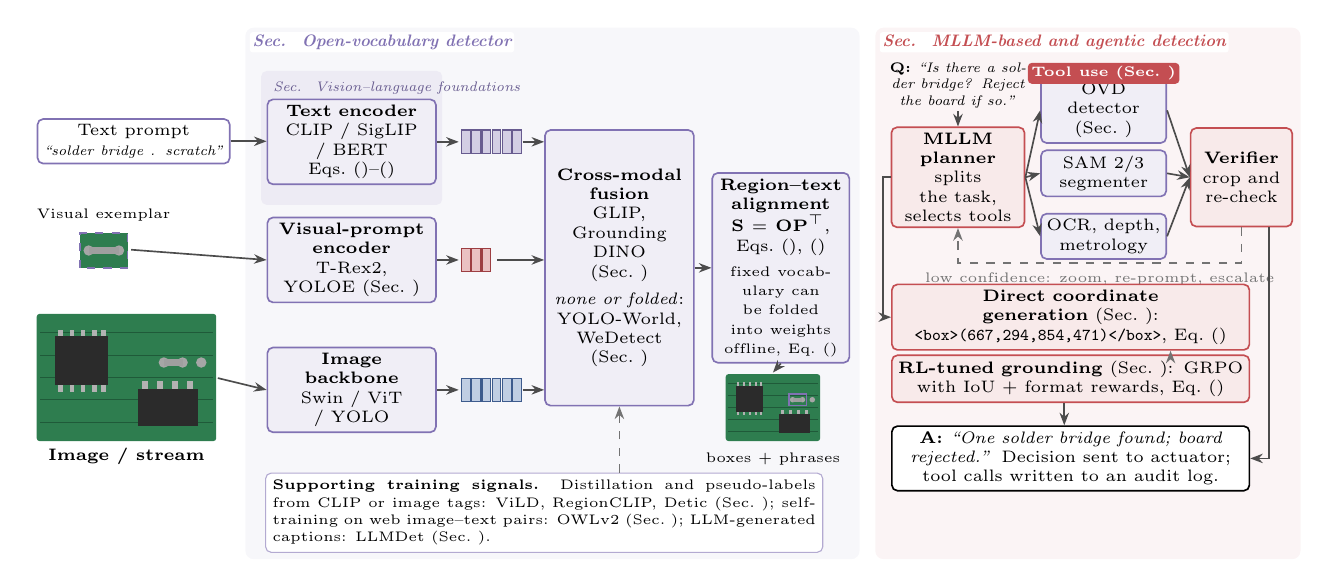
\begin{tikzpicture}[
  font=\fontsize{6}{7}\selectfont,
  mod/.style={draw=#1, fill=#1!12, rounded corners=2pt, line width=0.6pt, align=center, inner sep=2pt},
  tag/.style={fill=#1, text=white, rounded corners=1.5pt, font=\fontsize{5}{5.8}\selectfont\bfseries, inner sep=1.3pt, align=center},
  sec/.style={font=\fontsize{6}{7}\selectfont\bfseries\itshape, text=#1, anchor=north west, inner sep=1pt, fill=white, rounded corners=1pt},
  arr/.style={-{Stealth[length=1.6mm]}, line width=0.6pt, black!70},
  darr/.style={-{Stealth[length=1.6mm]}, line width=0.6pt, dashed, black!55},
  note/.style={font=\fontsize{5.3}{6.3}\selectfont, align=justify, text width=#1, inner sep=0pt},
  tok/.style={draw=#1!80!black, fill=#1!35, minimum width=0.11cm, minimum height=0.3cm, inner sep=0pt},
]
% ================= inputs
\node[mod=cOvd, fill=white, text width=2.3cm, anchor=north west] (tp) at (0,5.05) {Text prompt\\\mbox{\fontsize{5.5}{6.5}\selectfont\textit{``solder bridge . scratch''}}};
\begin{scope}[shift={(0.55,3.15)}, scale=0.55]
  \fill[pcbG] (0,0) rectangle (1.1,0.8); \fill[gray!70] (0.2,0.4) circle (0.12); \fill[gray!70] (0.9,0.4) circle (0.12); \fill[gray!75] (0.2,0.33) rectangle (0.9,0.47);
  \draw[cOvd, dashed, line width=0.6pt] (0,0) rectangle (1.1,0.8);
\end{scope}
\node[font=\fontsize{5.3}{6}\selectfont, anchor=south] at (0.85,3.62) {Visual exemplar};
\begin{scope}[shift={(0,0.95)}, scale=0.95] \scenePCB \end{scope}
\node[font=\fontsize{5.6}{6}\selectfont\bfseries] at (1.14,0.75) {Image / stream};
% ================= Section 4 region
\fill[cOvd!6, rounded corners=3pt] (2.65,-0.55) rectangle (10.45,6.2);
\node[sec=cOvd] at (2.7,6.15) {Sec.~\ref*{sec:ovd} Open-vocabulary detector};
% encoders (4.1)
\fill[cOvd!14, rounded corners=2pt] (2.85,3.95) rectangle (5.15,5.65);
\node[font=\fontsize{5}{5.5}\selectfont\itshape, text=cOvd!80!black, anchor=north west] at (2.88,5.63) {Sec.~\ref*{sec:vlfound} Vision--language foundations};
\node[mod=cOvd, text width=2.0cm] (te) at (4.0,4.75) {\textbf{Text encoder}\\CLIP / SigLIP / BERT\\Eqs.~(\ref*{eq:infonce})--(\ref*{eq:siglip})};
\node[mod=cOvd, text width=2.0cm] (ve) at (4.0,3.25) {\textbf{Visual-prompt encoder}\\T-Rex2, YOLOE (Sec.~\ref*{sec:ovd-unified})};
\node[mod=cOvd, text width=2.0cm] (ib) at (4.0,1.6) {\textbf{Image backbone}\\Swin / ViT / YOLO};
\draw[arr] (tp.east) -- (te.west |- tp.east);
\draw[arr] (1.2,3.38) -- (ve.west);
\draw[arr] (2.3,1.75) -- (ib.west);
% token strips
\foreach \i in {0,...,5}{\node[tok=cOvd] at (5.45+\i*0.13,4.75) {};}
\foreach \i in {0,...,2}{\node[tok=cAgent] at (5.45+\i*0.13,3.25) {};}
\foreach \i in {0,...,5}{\node[tok=cTwo] at (5.45+\i*0.13,1.6) {};}
\draw[arr] (te.east) -- (5.36,4.75); \draw[arr] (ve.east) -- (5.36,3.25); \draw[arr] (ib.east) -- (5.36,1.6);
% fusion (4.3) and real-time (4.5)
\node[mod=cOvd, text width=1.75cm, minimum height=3.5cm] (fu) at (7.4,3.15) {\textbf{Cross-modal}\\\textbf{fusion}\\GLIP,\\Grounding DINO\\(Sec.~\ref*{sec:ovd-grounding})\\[3pt]\textit{none or folded}:\\YOLO-World,\\WeDetect (Sec.~\ref*{sec:ovd-rt})};
\draw[arr] (6.17,4.75) -- (fu.west |- 0,4.75); \draw[arr] (5.85,3.25) -- (fu.west |- 0,3.25); \draw[arr] (6.17,1.6) -- (fu.west |- 0,1.6);
% alignment head
\node[mod=cOvd, text width=1.6cm, minimum height=1.6cm] (al) at (9.45,3.15) {\textbf{Region--text alignment}\\$\mathbf{S}=\mathbf{O}\mathbf{P}^{\top}$, Eqs.~(\ref*{eq:ovd}), (\ref*{eq:glip})\\[2pt]{\fontsize{5}{5.8}\selectfont fixed vocabulary can be folded into weights offline, Eq.~(\ref*{eq:reparam})}};
\draw[arr] (fu.east) -- (al.west);
% supporting band (4.2, 4.4)
\node[draw=cOvd!60, fill=white, rounded corners=2pt, note=6.9cm, inner sep=2.5pt, anchor=north west] (sup) at (2.9,0.55) {\textbf{Supporting training signals.} Distillation and pseudo-labels from CLIP or image tags: ViLD, RegionCLIP, Detic (Sec.~\ref*{sec:ovd-distill}); self-training on web image--text pairs: OWLv2 (Sec.~\ref*{sec:ovd-owl}); LLM-generated captions: LLMDet (Sec.~\ref*{sec:ovd-grounding}).};
\draw[darr] (sup.north -| fu.south) -- (fu.south);
% detector output
\begin{scope}[shift={(8.75,0.95)}, scale=0.5]
  \scenePCB \draw[bx=cOvd, line width=0.6pt] (1.6,0.9) rectangle (2.05,1.2);
\end{scope}
\draw[arr] (al.south) -- (9.35,1.82);
\node[font=\fontsize{5}{5.5}\selectfont, align=center] at (9.35,0.72) {boxes + phrases};
% ================= Section 5 region
\fill[cAgent!6, rounded corners=3pt] (10.65,-0.55) rectangle (16.05,6.2);
\node[sec=cAgent] at (10.7,6.15) {Sec.~\ref*{sec:agentic} MLLM-based and agentic detection};
\node[mod=cAgent, text width=1.55cm, minimum height=1.25cm] (pl) at (11.7,4.3) {\textbf{MLLM planner}\\splits the task,\\selects tools};
\node[mod=cOvd, text width=1.45cm] (t1) at (13.55,5.15) {OVD detector\\(Sec.~\ref*{sec:ovd})};
\node[mod=cOvd, text width=1.45cm] (t2) at (13.55,4.35) {SAM 2/3 segmenter};
\node[mod=cOvd, text width=1.45cm] (t3) at (13.55,3.55) {OCR, depth, metrology};
\node[tag=cAgent] at (13.55,5.62) {Tool use (Sec.~\ref*{sec:mllm-tools})};
\foreach \t in {t1,t2,t3}{\draw[arr] (pl.east) -- (\t.west);}
\node[mod=cAgent, text width=1.15cm, minimum height=1.25cm] (vf) at (15.3,4.3) {\textbf{Verifier}\\crop and re-check};
\foreach \t in {t1,t2,t3}{\draw[arr] (\t.east) -- (vf.west);}
\draw[darr] (vf.south) -- ++(0,-0.45) -| node[pos=0.25, below, font=\fontsize{4.6}{5}\selectfont]{low confidence: zoom, re-prompt, escalate} (pl.south);
% 5.1 direct and 5.2 RL
\node[mod=cAgent, text width=4.4cm, anchor=north west] (dg) at (10.85,2.95) {\textbf{Direct coordinate generation} (Sec.~\ref*{sec:mllm-direct}): \texttt{<box>(667,294,854,471)</box>}, Eq.~(\ref*{eq:mllm-box})};
\node[mod=cAgent, text width=4.4cm, anchor=north west] (rl) at (10.85,2.05) {\textbf{RL-tuned grounding} (Sec.~\ref*{sec:mllm-rl}): GRPO with IoU + format rewards, Eq.~(\ref*{eq:grpo})};
\draw[arr] (pl.west) -- ++(-0.1,0) |- (dg.west);
\draw[darr] (rl.north -| 14.4,0) -- (dg.south -| 14.4,0);
% answer
\node[mod=black, fill=white, text width=4.4cm, anchor=north west] (ans) at (10.85,1.15) {\textbf{A:} \textit{``One solder bridge found; board \mbox{rejected}.''} Decision sent to \mbox{actuator}; tool calls written to an audit log.};
\draw[arr] ([xshift=0.35cm]vf.south) |- (ans.east);
\draw[arr] (rl.south -| 13.05,0) -- (ans.north -| 13.05,0);
\node[font=\fontsize{5.2}{6}\selectfont, align=center, text width=1.9cm, anchor=north, inner sep=1pt] (q) at (11.7,5.8) {\textbf{Q:} \textit{``Is there a solder bridge? Reject the board if so.''}};
\draw[arr] (q.south) -- (pl.north);
\end{tikzpicture}

\end{document}
